\documentclass{article}
\usepackage[utf8]{inputenc}
\usepackage{amsmath}
\usepackage{graphicx}
\usepackage{float}
\usepackage{amssymb}
\usepackage{listings}
\usepackage{pgfplots}
\usepackage{siunitx}

\usepackage{tabularx}
\usepackage{ragged2e}
\usepackage{multirow}

\pgfplotsset{compat=1.15}
\title{ITIA Target Programming (Robot) Lab Report}
\author{Stefan Adelmann (01633044) and Hannes Brantner (01614466)}
\begin{document}
\maketitle{}
\clearpage{}
\section{SysML Review}
For the robot station in phase 2, no two SysML models had to be merged. The presented model from phase 1 of this lecture contains the whole station. As a self review we remodeled certain aspects of the robot station.

\subsection{Parametric diagram}
The parametric diagram that was created in phase 1 has no direct link to the real robot station. Distances do not need to be handled by the user in any way and the robot itself has sophisticated movement schemes  pre-installed. Measurements between two points in 3D space therefore cannot be seen as a straight line. The diagram was dropped from the revised SysML model.

\subsection{Internal Block Diagram}
The diagram does not show the internal wiring of individual sensors and actuators. This was an deliberate choice to not overcrowd the diagram. Information on the internal wiring of the used connectors can be found in separate tables.


\section{I/O Mapping}
The following I/O mapping was created for the robot station.

\subsection{Robot}
Movement of the 6 axis robot arm, shown in \ref{fig:robot_axis} as well as the function of the multi-functional gripper is handled internally by the robot controller. The user does not need to define these I/O mapping themselves, instead the programming language Melfa uses commands shown in table \ref{tab:robot_ctrl} to actuate the arm. Additionally OPC UA methods are shown that execute the corresponding action.
\begin{figure}[htp]
	\centering
	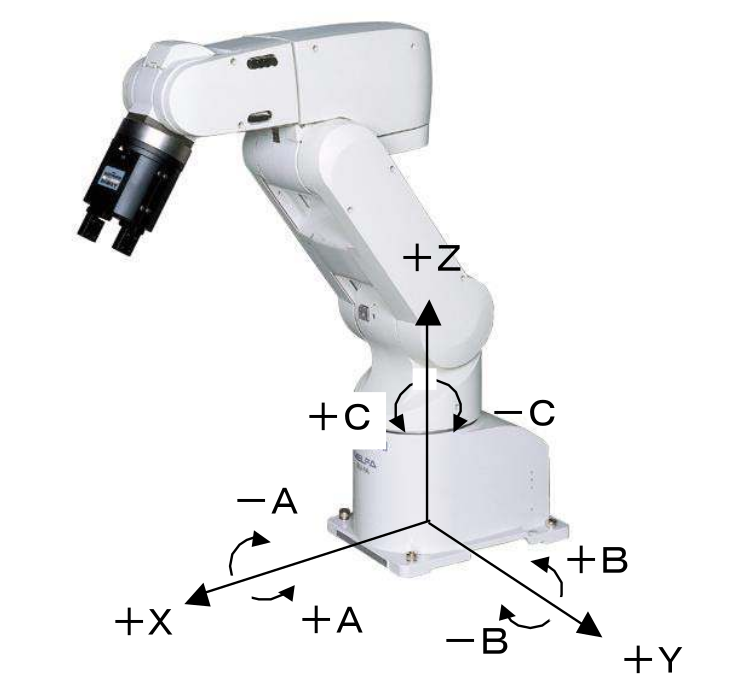
\includegraphics[width=0.6\textwidth]{images/robot_axis.png}
	\caption{Robot coordinate system in XYZ mode}
	\label{fig:robot_axis}
\end{figure}

\begin{center}
	\setlength\extrarowheight{4pt}
	\small
	\begin{table}[h]
		\begin{tabularx}{\textwidth}{|p{3cm}|p{4cm}|X|}
			\hline
			\multicolumn{3}{|c|}{\bf \color{white} \large Gripper}\\
			\hline\hline
			\bf Melfa-Command & \bf OPC UA & \bf Beschreibung\\
			\hline\hline
			Mov(X,Y,Z,A,B,C) & move(X,Y,Z,A,B,C) & Modul Roboter (Hand) - Position, Rotation anfahren\\
			\hline
			HOpen 1 & gripperOpen() & Modul Roboter (Hand) - Gripper öffnen\\
			\hline
			HClose 1 & gripperClose() & Modul Roboter (Hand) - Gripper schließen\\
			\hline
		\end{tabularx}
		\label{tab:robot_ctrl}
	\end{table}
	
\end{center}

\subsection{Robot Control}
The robot station is controlled by a controller that is programmed via the Melfa programming language. 
\begin{center}
	\begin{table}[h]
		\begin{tabular}[h]{|p{1.2cm}p{5.5cm}|}
			\hline
			\multicolumn{2}{|c|}{\bf Controller}\\
			\hline\hline
			Device: & Robot Controller\\
			\hline
			ID: & CR750-D\\
			\hline
			MAC: & \\
			\hline
			IP: & 192.168.162.82/25\\
			\hline
		\end{tabular} \\
		\label{tab:controller}
	\end{table}
\end{center}

The user can execute commands and movements of the robot station via an OPC Ua server running on a Raspberry Pi. 

\begin{center}
	%\scriptsize
	\setlength\extrarowheight{2pt}

	\begin{table}[h]
			\begin{tabular}[h]{|p{1.2cm}p{4.5cm}|}
			\hline
			\multicolumn{2}{|c|}{\bf OPC UA Gateway}\\
			\hline\hline
			Device: & RaspberryPi 3\\
			\hline
			ID: & BCM2835 (a02082)\\
			\hline
			MAC: & b8:27:eb:09:db:ca\\
			\hline
			IP: & 192.168.162.84/25\\
			\hline
		\end{tabular} 
		\label{tab:robot_raspi}
	\end{table}
	

\end{center}

\subsection{Sensors/Actuators}
The robot controller addresses in and outputs via an index. Every sensor or actuator that is connected to the robot can be read and set 
\begin{center}

	\setlength\extrarowheight{4pt}
	\small
	\begin{tabularx}{\textwidth}{|p{1cm}|X|}
		\hline
		\multicolumn{2}{|c|}{\bf \color{white} \large Sensoren}\\
		\hline\hline
		\bf Index & \bf Beschreibung\\
		\hline\hline
		1 & Modul Roboterhandling - Werkstück ausgerichtet\\
		\hline
		2 & Modul Roboterhandling - Werkstück in Abholposition\\
		\hline
		3 & Bedienfeld - Start (Schließer)\\
		\hline
		4 & Bedienfeld - Stopp (Öffner) \\
		\hline
		5 & Bedienfeld - Reset (Schließer)\\
		\hline
		7 & Bedienfeld - COM Brücke (I7)\\
		\hline
		8 & Modul Robotermontage (Federmagazin) - Schieber eingefahren\\
		\hline
		9 & Modul Robotermontage (Federmagazin) - Schieber ausgefahren\\
		\hline
		10 & Modul Robotermontage (Federmagazin) - Feder vorhanden \\
		\hline
		12 & Modul Robotermontage (Deckelmagazin) - Schieber eingefahren\\
		\hline
		13 & Modul Robotermontage (Deckelmagazin) - Schieber ausgefahren\\
		\hline
		15 & Modul Robotermontage (Deckelmagazin) - Deckel auf Ablage\\
		\hline
		900 & Modul Roboter (Hand) - Teil nicht schwarz\\
		\hline
	\end{tabularx}
\end{center}


\begin{center}
	\setlength\extrarowheight{4pt}
	\small
	\begin{tabularx}{\textwidth}{|p{1cm}|X|}
		\hline

		\multicolumn{2}{|c|}{\bf \color{white} \large Aktoren}\\
		\hline\hline

		\bf Index & \bf Beschreibung\\
		\hline\hline
		0 & Bedienfeld - Start (LED)\\
		\hline
		1 & Bedienfeld - Reset (LED)\\
		\hline
		2 & Bedienfeld - Q1 (LED)\\
		\hline
		3 & Bedienfeld - Q2 (LED)\\
		\hline
		4 & Bedienfeld - COM Brücke (Q4)\\
		\hline
		8 & Modul Robotermontage (Federmagazin) - Schieber ausfahren\\
		\hline
		12 & Modul Robotermontage (Deckelmagazin) - Schieber ausfahren\\
		\hline
	\end{tabularx}
\end{center}
\newpage

\section{Handover Protocol}
Since the robot station by itself is capsuled no handover protocol between the internal modules is necessary. The robot can however be used in combination with other stations via the OPC Ua interfaced that was created in this phase. A Raspberry Pi is used as a OPC Ua server connected to the robot controller via a telnet interface. This setup provides the following methods:

\begin{center}
	\setlength\extrarowheight{4pt}
	\small
	\begin{tabularx}{\textwidth}{|p{5cm}|X|}
		\hline
		
		\multicolumn{2}{|c|}{\bf \color{white} \large Aktoren}\\
		\hline\hline
		
		\bf Method & \bf Function\\
		\hline\hline
		OpenGripper() & Opens the multi function gripper\\
		\hline
		CloseGripper() & Closes the multi function gripper\\
		\hline
		Move(X,Y,Z,A,B,C) & Moves the robot arm to the given coordinates\\
		\hline
		GetErrorLog(NUMLOGS) & Returns the last NUMLOGS errors that occurred\\
		\hline
		ReadInput(INDEX) & Returns the state of the input at the given index\\
		\hline
		WriteOutput(INDEX, STATE) & Sets the output at the given INDEX to the given STATE\\
		\hline
		ResetError() & Resets the robot controller from the error state\\
		\hline
	\end{tabularx}
\end{center}

\end{document}
